\documentclass[matan.tex]{subfiles}

 
\begin{document}
 
\begin{lect}{18.10.19}
    
    \begin{Definition}
        \[E \subset \R^2 \text{ - не замк. и не огр } \qq f \text{ - непр}\]
        \[\exists \sup_{(x, y) \in E} f(x, y) \qq \inf_{(x, y) \in E} f(x, y)\]
        \begin{figure}[H]
            \includegraphics[width=7cm]{pics/8}
            \centering
        \end{figure}
        \[\exists \ (x_n, y_n) \in E : f(x_n, y_n) \to \sup f\]
        \[\exists \{(x_{n_k}, y_{n_k}  )\}\]
        \[x_{n_k} \to  a, \q y_{n_k} \to b\]
        \[x_{n_k} \to  a, \q y_{n_k} \to \pm \infty\]
        \[x_{n_k} \to +\infty, \q y_{n_k} \to b\]
        \[x_{n_k}  \to \pm \infty, \q y_{n_k}  \to \pm \infty\]
        \[x_{n_k} \to -\infty, \q y_{n_k} \to b\]
        Если $(a, b) \in E$, то $f(x_{n_k} , y_{n_k} ) \to f(a, b)$\\
        т.е $f(a, b) = \sup = \max$\\
        \\
        Если $(a, b) \cancel{\in } E$, то $(a, b) \in \us{\text{Граница}}{\text{Fr E}}$
        \[f(x_{n_k}, y_{n_k} ) \to \lim_{(x,y) \to (a, b)} f(x, y) = \sup f \]
        \[\us{\begin{matrix}
            x_{n_k} \to  + \infty\\
            y_{n_{k} } \to b
        \end{matrix}}{f(x_{n_k}, y_{n_k} )} \to  \lim_{\begin{matrix}
            x \to +\infty\\
            y \to b
        \end{matrix}} f(x, y)\]
        Подозр. точки
        \begin{enumerate}
            \item Внутри
                \[\begin{cases}
                    f'_x = 0\\
                    f'_y = 0
                \end{cases}\]
            \item На уч-ке $\Phi_1(x, y) = 0$
                \[\rk \Phi_1' < 1\]
                \[\text{ или } \LL = f - \lambda \Phi_1\]
            \item На участке $\Phi_2(x, y) = 0$
                \[\lim_{\begin{matrix}
                    x \to a\\
                    y \to b
            \end{matrix}} f(x, y) = f(a, b)\]
            \[\LL = f(a, b) - \lambda \Phi_2(a, b)\]
            \item $\displaystyle \lim_{\begin{matrix}
                x \to a\\
                y \to +\infty
            \end{matrix}} f(x, y) $
            \[\lim_{\begin{matrix}
                x \to +\infty\\
                y \to b
        \end{matrix}}f(x, y) \]
            \[\lim_{\begin{matrix}
                x \to +\infty\\
                y \to +\infty
        \end{matrix}} f(x, y)\]
        \end{enumerate}
        Если наиб - предел, то $\sup$ не достигается, иначе достигается
    \end{Definition}

    \begin{Task}[1]
        \[f(x, y) = (x^2 + y^2)e^{-x-2y} \]
        \[\sup, \inf \text{ на множестве } E = \{(x, y)| \ x \geq 0, \ t > \frac{3}{5}\}\]
        \begin{figure}[H]
            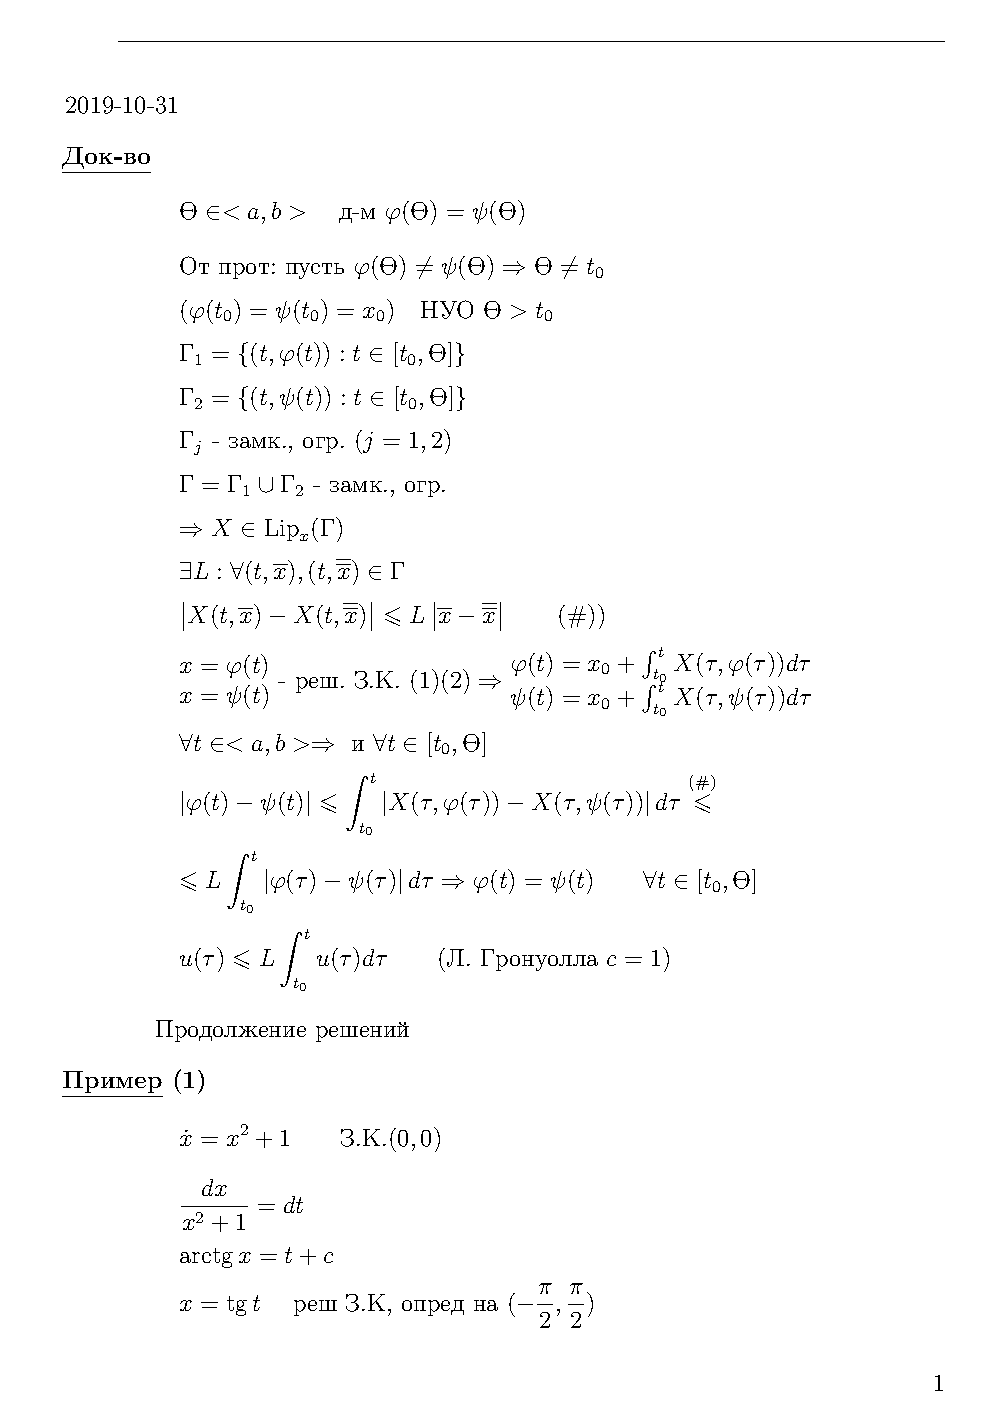
\includegraphics[width=7cm]{pics/9}
            \centering
        \end{figure}
        
        \[1) \text{ внутри}\]
        \[\begin{cases}
            f'_x = 2xe^{-x-2y} - (x^2 + y^2)e^{-x - 2y} = 0\\
            f'_y = 2ye^{-x-2y} - 2(x^2 + y^2)e^{-x - 2y} = 0 
        \end{cases}\]
        \[e^{-x-2y} \neq 0 \q поделим\]
        \[\begin{cases}
            2x - (x^2 + y^2) = 0\\
            2y - 2(x^2 + y^2) = 0
        \end{cases}\]
        \[\begin{cases}
            2x = x^2 + y^2\\
            y = x^2 + y^2
        \end{cases}\]
        \[y = 2x\]
        \[2x = x^2 + 4x^2\]
        \[5x^2 - 2x = 0\]
        \[x(5x - 2) = 0\]
        \[\begin{cases}
            x = 0\\
            y = 0
        \end{cases} \cancel{\in } E \text{ и не явл. границей}\]
        \[\begin{cases}
            x = \frac{2}{5}\\
            y = \frac{4}{5}
        \end{cases} \in E\]
        \[2) \text{ на участке } x = 0, \q y > \frac{3}{5}\]
        \[\text{Просто подставим } x = 0 \q \text{(можно без ф. Лагранжа)}\]
        \[f(0, y) = y^2e^{-2y} \]
        \[f' = 2ye^{-2y} - 2y^2e^{-2y} = 0 \qq e^{-2y} \neq 0 \q \text{ делим}\]
        \[2y - 2y^2 = 0\]
        \[y(1 - y) = 0\]
        \[y = 0 \ \cancel{\in }\ E\]
        \[\begin{cases}
            y = 1\\
            x = 0
        \end{cases} \in E\]
        \[3) \text{ на участке границы } y = \frac{3}{5}, \ x \geq 0\]
        т.к непр на все плоск.
        \[\lim_{\begin{matrix}
            x \to a\\
            y \to \frac{3}{5}
        \end{matrix}} (x^2 + y^2)e^{-x-2y} = (a^2 + \frac{9}{25}) e^{-a-\frac{6}{5}}  \qq 
        a \geq 0\]
        \[((a^2 + \frac{9}{25})e^{-\frac{5}{9}} e^{-a}  )' = e^{-\frac{6}{5}} 
        (2ae^{-a} - (a^2 + \frac{9}{25})e^{-a}  ) = 0\]
        \[2a - a^2 - \frac{9}{25} = 0\]
        \[25a^2 - 50a + 9 = 0\]
        \[d = 2500 - 900 = 400^2\]
        \[a_{1,2} = \frac{50 \pm 40}{50} = \frac{9}{5}, \q \frac{1}{5} \]
        \[\begin{cases}
            a = \frac{1}{5}\\
            y = \frac{3}{5}
        \end{cases} \qq \begin{cases}
            a = \frac{9}{5}\\
            y = \frac{3}{5}
        \end{cases}\]
        \[4) \text{ угловые точки}\]
        \[(0, \frac{3}{5}) \text{ на границе, не берем}\]
        Значения:
        \[f(\frac{2}{5}, \frac{4}{5}) = (\frac{4}{25} + \frac{16}{25})e^{-\frac{2}{5} - 
        \frac{8}{5}} = \frac{4}{5}e^{-2} \approx 0,108\]
        \[f(0, 1) = (0 + 1)e^{-0 -2} = e^{-2} \approx 0,135.. \]
            т.к. $f $ -непр $\Ra $ предел = значению
        \[\lim_{\begin{matrix}
            x \to \frac{1}{5}\\
            y \to \frac{3}{5}
        \end{matrix}} f(x, y) = (\frac{1}{25}
        = \frac{9}{25})e^{-\frac{1}{5} - \frac{6}{5}} =
        \frac{2}{5}e^{-\frac{7}{5}} \approx 0,099.. \]
        \[\lim_{\begin{matrix}
            x \to \frac{9}{5}\\
            y \to \frac{3}{5}
    \end{matrix}} f(x, y) = (\frac{81}{25} + \frac{9}{25})e^{-\frac{9}{5} - \frac{6}{5}} 
    = \frac{18}{5} e^{-3} \approx 0,1792\]
    \[ \text{(т.к предел, то $\sup$ не достигается)}\]
    \[\lim_{\begin{matrix}
        x \to 0\\
        y \to \frac{3}{5}
    \end{matrix}} f(x, y) = (0 + \frac{9}{25})e^{- 0 - \frac{6}{5}} =
    \frac{9}{25}e^{-\frac{6}{5}} \approx 0,1084...   \]
    \[\lim_{\begin{matrix}
        x \to +\infty\\
        y \to b
    \end{matrix}} = \lim_{\begin{matrix}
        x \to +\infty\\
        y \to b
    \end{matrix}} (x^2e^{-x}e^{-2y} + y^2e^{-x} e^{-2y}) = 0 \]
    \[\lim_{\begin{matrix}
        x \to a\\
        y \to +\infty
    \end{matrix}} f(x, y) = \lim_{\begin{matrix}
    x \to a\\
    y \to +\infty
    \end{matrix}}(x^2e^{-x}e^{-2y} + y^2e^{-2y}e^{-x}) = 0\]
    \[\lim_{\begin{matrix}
        x \to +\infty\\
        y \to +\infty
    \end{matrix}} f(x, y) = \lim_{\begin{matrix}
    x \to +\infty\\
    y \to +\infty
    \end{matrix}} (x^2e^{-x}e^{-2y} + y^2e^{-2y}e^{-x}) = 0 \]
    Наим - 0 - $\inf$ (не достиг., т.к. предел)
    \[0 < (x^2 + y^2)e^{-x-2y} < \frac{18}{5}e^{-3}  \]
    \[(x, y) \in E\]
    \end{Task}

    \begin{task}[2]
        При каких размерах открытая коробка постоянного объема имеет наим. поверхность?
        \begin{figure}[H]
            \includegraphics[width=7cm]{pics/10}
            \centering
        \end{figure}
        \[1. \text{ постановка задачи}\]
        \[S = xy + 2xz + 2yz \qq x > 0 \q y > 0 \q z > 0\]
        \[V = xyz = const\]
        \[\Phi = xyz - V = 0\]
        \[\Phi' = \begin{pmatrix}
            yz, & xz, & xy
        \end{pmatrix}\]
        \[\rk \Phi' = 1\]
        \[\LL = xy + 2xz + 2yz - \lambda(xyz - V)\]
        На этой пов-ти
        \begin{figure}[H]
            \includegraphics[width=7cm]{pics/11}
            \centering
        \end{figure}
        \[\lim_{\begin{matrix}
            x \to +\infty\\
            y \to 0+\\
            z \to ?
        \end{matrix}} S = ?\]
        \[2. \text{ постановка задачи}\]
        \[z = \frac{V}{xy}\]
        \[S = xy + 2x \cdot \frac{V}{xy} + 2y \cdot \frac{V}{xy} = 
        xy + \frac{2V}{y} + \frac{2V}{x}\]
        \[\text{Наим значение } S \text{ в обл. } \begin{cases}
            x > 0\\
            y > 0
        \end{cases}\]
        \begin{figure}[H]
            \includegraphics[width=7cm]{pics/12}
            \centering
        \end{figure}
        
        \[1) \text{ Внутри}\]
        \[\begin{cases}
            f'_x = y - \frac{2V}{x^2} = 0\\
            f'_y = x - \frac{2V}{y^2} = 0
        \end{cases}\]
        \[y = \frac{2V}{x^2}\]
        \[x - \frac{2Vx^2}{4V^2} = 0\]
        \[1 - \frac{x^3}{2V} = 0\]
        \[x^3 = 2V\]
        \[x = \sqrt[3]{2V}\]
        \[y = \frac{2V}{(2V)^{\frac{2}{3}} } = \sqrt[3]{2V}\]
        \[S(\sqrt[3]{2V}, \sqrt[3]{2V}) = \sqrt[3]{4V^2} + \frac{2V}{\sqrt[3]{2V}} + 
        \frac{2V}{\sqrt[3]{2V}} = \sqrt[3]{4V^2} + 2 \sqrt[3]{4V^2} = 3\sqrt[3]{4V^2}\]
        \[2)\]
        \[\lim_{\substack{x \to a\\ y \to 0+}}
        (xy + \frac{2V}{y} + \frac{2V}{x}) = +\infty\]
        \[\lim_{\substack{x \to 0+ \\ y \to a}}(xy + \frac{2V}{y} + \frac{2V}{x}) = 
        +\infty\]
        \[\lim_{\substack{x \to 0+ \\ y \to 0 +}} (xy + \frac{2V}{y} + \frac{2V}{x}) =
        +\infty\]
        \[\lim_{\substack{x \to a > 0\\ y \to +\infty}}(xy + \frac{2V}{y} + \frac{2V}{x})
        = + \infty\]
        \[\lim_{\substack{x \to +\infty \\ y \to a > 0}}(xy + \frac{2V}{y} + \frac{2V}{x})
        = + \infty\]
        \[\lim_{\substack{x \to +\infty \\ y \to +\infty}}(xy + \frac{2V}{y} +
        \frac{2V}{x}) = +\infty \]
        \[\lim_{\substack{x \to 0+ \\ y \to +\infty}} (xy + \frac{2V}{y} + \frac{2V}{x}) =
        +\infty\]
        Наим. знач $3\sqrt[3]{4V^2}$
        \[x = \sqrt[3]{2V}\]
        \[y = \sqrt[3]{2V}\]
        \[z = \frac{V}{\sqrt[3]{V^2}} = \sqrt[3]{\frac{1}{4}V}\]
    \end{task}
\end{lect}

\end{document}
